%\newcommand{\Exp}{\Exp}
\allowdisplaybreaks

% Syntax: \colorboxed[<color model>]{<color specification>}{<math formula>}
\newcommand*{\colorboxed}{}
\def\colorboxed#1#{%
	\colorboxedAux{#1}%
}

\newcommand*{\colorboxedAux}[3]{%
	% #1: optional argument for color model
	% #2: color specification
	% #3: formula
	\begingroup
	\colorlet{cb@saved}{.}%
	\color#1{#2}%
	\boxed{%
		\color{cb@saved}%
		#3%
	}%
	\endgroup
}

% reset section counter
\setcounter{section}{0}

%\metadata{lecture ID}{Your names}{date}
\metadata{2}{Anna Shors}{April 9th, 2021}

\sec{Review and overview}

In the last lecture, we introduced the idea of nonparametric regression including the regressogram, local averaging, and Naradaya-Watson kernel estimators. 

In this lecture, we expand on the ideas introduced in the first lecture. We discuss the bias-variance trade-off and its implications in the nonparametric setting, citing a formal theorem. We next introduce the concept of linear smoothers as a way to unify many common nonparametric regression methods and conclude with an introduction to another approach to nonparametric regression: local linear regression. We discuss how local linear regression overcomes some of the challenges faced by kernel estimators. 

\sec{Example: the optimal bandwidth}

Consider the function $r(x)$, along with the given data points, shown in the plot below:

\begin{center}
	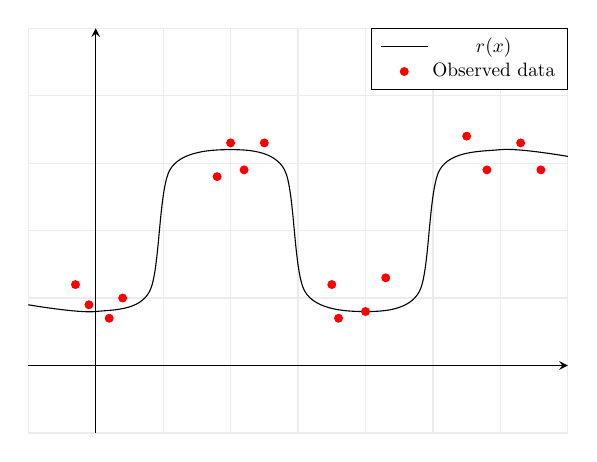
\begin{tikzpicture}[scale=1]
		\begin{axis}[
			ticks=none,
			xtick distance=1,
			ytick distance=1,
			axis equal image=true,
			grid,
			grid style={gray!15},
			grid=both,
			axis lines=middle,
			xmin=-1, xmax=7, ymin=-1, ymax=5,
			axis x line=center,
			axis y line=center,
			legend style={nodes={scale = 0.7}, at={(1,1)},anchor=north east}
			]
			\addplot[smooth] plot coordinates
			{
				(-1,0.9) 
				(0,0.8) 
				(0.8, 1.1) 
				(1.1, 2.9) 
				(2, 3.2)
				(2.8, 2.9)
				(3.1, 1.1)
				(4, 0.8) 
				(4.8, 1.1)
				(5.1, 2.9)
				(6, 3.2)
				(7, 3.1)
			};
			\addlegendentry{$r(x)$}
			\addplot[only marks, color=red, mark options={scale=0.7}] coordinates
			{
				(-0.1, 0.9)
				(0.2, 0.7)
				(-0.3, 1.2)
				(0.4, 1)
				
				(2, 3.3)
				(2.2, 2.9)
				(1.8, 2.8)
				(2.5, 3.3)
				
				(3.6, 0.7)
				(3.5, 1.2)
				(4, 0.8)
				(4.3, 1.3)
				
				(5.5, 3.4)
				(5.8, 2.9)
				(6.3, 3.3)
				(6.6, 2.9)
			};
			\addlegendentry{Observed data}
			
		\end{axis}
		
	\end{tikzpicture}
\end{center}

\noindent We would like to use local averaging to estimate $r(x_i)$ at each data point $x_i$. We consider three choices for the bandwidth $h$.
\begin{enumerate}
	\item $h = \infty$: when $h$ is infinite, we simply average over all data points in the dataset when making a prediction for a given point $x$. Thus, the resulting estimator $\hat r$ is simply a constant function, as shown in blue below:
	
	
	\begin{center}
		
		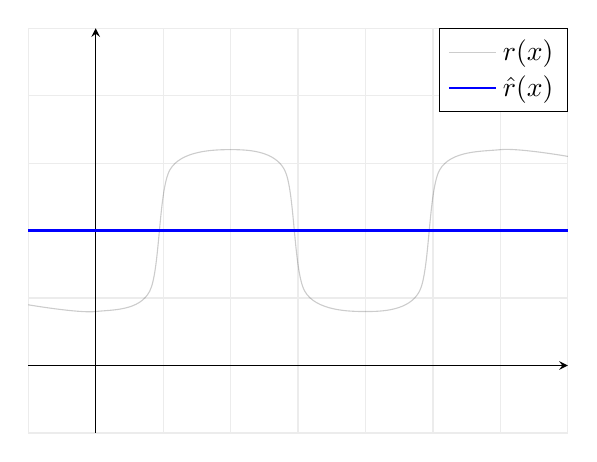
\begin{tikzpicture}[scale=1]
			\begin{axis}[
				ticks=none,
				xtick distance=1,
				ytick distance=1,
				axis equal image=true,
				grid,
				grid style={gray!15},
				grid=both,
				axis lines=middle,
				xmin=-1, xmax=7, ymin=-1, ymax=5,
				axis x line=center,
				axis y line=center,
				legend style={at={(1,1)},anchor=north east}
				]
				\addplot[smooth, opacity = 0.2] plot coordinates
				{
					(-1,0.9) 
					(0,0.8) 
					(0.8, 1.1) 
					(1.1, 2.9) 
					(2, 3.2)
					(2.8, 2.9)
					(3.1, 1.1)
					(4, 0.8) 
					(4.8, 1.1)
					(5.1, 2.9)
					(6, 3.2)
					(7, 3.1)
				};
				\addlegendentry{$r(x)$}
				
				\addplot[thick, smooth, color=blue] plot coordinates
				{
					(-1, 2)
					(0,2)
					(1,2)
					(2,2)
					(4,2)
					(5,2)
					(6,2)
					(7,2)
				};
				\addlegendentry{$\hat r(x)$}
				
			\end{axis}
			
		\end{tikzpicture}
	\end{center}
	
	$h = \infty$ is clearly undesirable in this example, because $\hat r(x)$ carries no information about the underlying function $r(x)$.
	\item $h = 0$: the only data point $x_i$ that satisfies $|x-x_i| \leq h$ is $x$ itself. Thus, for a given $x_i$ in the training set, the predicted value of $r(x_i)$ will be precisely equal to the observed outcome $Y_i$ (i.e. $\hat r(x_i) = Y_i$), so that we fail to denoise the dataset at all.
	% TODO: add plot!
	
	\begin{center}
		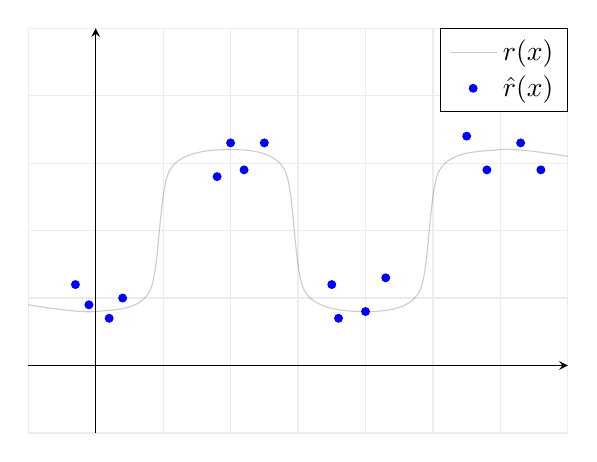
\begin{tikzpicture}[scale=1]
			\begin{axis}[
				ticks=none,
				xtick distance=1,
				ytick distance=1,
				axis equal image=true,
				grid,
				grid style={gray!15},
				grid=both,
				axis lines=middle,
				xmin=-1, xmax=7, ymin=-1, ymax=5,
				axis x line=center,
				axis y line=center,
				legend style={at={(1,1)},anchor=north east}
				]
				\addplot[smooth, opacity = 0.2] plot coordinates
				{
					(-1,0.9) 
					(0,0.8) 
					(0.8, 1.1) 
					(1.1, 2.9) 
					(2, 3.2)
					(2.8, 2.9)
					(3.1, 1.1)
					(4, 0.8) 
					(4.8, 1.1)
					(5.1, 2.9)
					(6, 3.2)
					(7, 3.1)
				};
				\addlegendentry{$r(x)$}
				\addplot[only marks, color=blue, mark options={scale=0.7}] plot coordinates
				{
					(-0.1, 0.9)
					(0.2, 0.7)
					(-0.3, 1.2)
					(0.4, 1)
					
					(2, 3.3)
					(2.2, 2.9)
					(1.8, 2.8)
					(2.5, 3.3)
					
					(3.6, 0.7)
					(3.5, 1.2)
					(4, 0.8)
					(4.3, 1.3)
					
					(5.5, 3.4)
					(5.8, 2.9)
					(6.3, 3.3)
					(6.6, 2.9)
				};
				\addlegendentry{$\hat r(x)$}
			\end{axis}
			
		\end{tikzpicture}
	\end{center}
	
	\item $h = 1$: This is the best choice for this example. $h=1$ has the effect of averaging only the nearby points when making a prediction on an example $x_i$. This is desirable because points substantially far from $x_i$ exhibit quite different behavior and thus should not influence the estimate of $r(x_i)$. $h=1$ has the effect of adequately denoising the data without smoothing the estimator $\hat r$ too severely, as the plot below illustrates.
	
	\begin{center}
		\begin{tikzpicture}[scale=1]
			\begin{axis}[
				ticks=none,
				xtick distance=1,
				ytick distance=1,
				axis equal image=true,
				grid,
				grid style={gray!15},
				grid=both,
				axis lines=middle,
				xmin=-1, xmax=7, ymin=-1, ymax=5,
				axis x line=center,
				axis y line=center,
				legend style={nodes={scale=0.7}, at={(1,1)},anchor=north east}
				]
				\addplot[thick, smooth, opacity = 0.2] plot coordinates
				{
					(-1,0.9) 
					(0,0.8) 
					(0.8, 1.1) 
					(1.1, 2.9) 
					(2, 3.2)
					(2.8, 2.9)
					(3.1, 1.1)
					(4, 0.8) 
					(4.8, 1.1)
					(5.1, 2.9)
					(6, 3.2)
					(7, 3.1)
				};
				\addplot[only marks, color=red, opacity = 0.2, mark options={scale=0.7}] plot coordinates
				{
					(-0.1, 0.9)
					(0.2, 0.7)
					(-0.3, 1.2)
					(0.4, 1)
					
					(2, 3.3)
					(2.2, 2.9)
					(1.8, 2.8)
					(2.5, 3.3)
					
					(3.6, 0.7)
					(3.5, 1.2)
					(4, 0.8)
					(4.3, 1.3)
					
					(5.5, 3.4)
					(5.8, 2.9)
					(6.3, 3.3)
					(6.6, 2.9)
				};
				\addlegendentry{$r(x)$}
				\addlegendentry{observed}
				\addplot[thick, smooth, color=blue] plot coordinates {
					(-0.5, 0.9)
					(0.7, 0.9)
					
					(1.6, 3.1)
					(2.7, 3.1)
					
					(3.3, 1)
					(4.5, 1)
					
					(5.3, 3.1)
					(6.8, 3.1)
				};
				\addlegendentry{$\hat r(x)$}
				
				\node[] at (120,80) {$x$};  
				\node[] at (75,30) {$h = 1$};  
				\draw[dashed] (120,100) -- (120,170);
				\draw[dashed, color=blue] (30,100) -- (30,180);
				\draw[dashed, color=blue] (220,100) -- (220,400);
				%\draw[dashed] (1.2,0.8) -- (1.2,4.7);
				\draw [decorate,decoration = {brace,amplitude=3pt,mirror}] (30,60) -- (120,60);
			\end{axis}
			
		\end{tikzpicture}
	\end{center}
	
\end{enumerate}

\sec{The bias-variance trade-off}
\subsec{Motivation for using MSE}
We begin with a motivation for why we use MSE to measure performance of an estimator. We claim that MSE is very closely related to predictive risk, which measures how well $\hat r(x)$ performs on a new observation (with fresh randomness). After creating our estimator $\hat r(x)$, let $Z_i = r(x_i) + \xi_i$, where $\xi_i$ has mean 0 and variance $\sigma^2$. Then,
\begin{align}
	\text{predictive risk}(\hat r) &\stackrel{\Delta}{=} \mathbb{E
	}_{Z_i}\biggl[\frac{1}{n}\sum_{i=1}^n (\hat r(x_i) - Z_i)^2\biggr] \nonumber \\
	&= \frac{1}{n}\sum_{i=1}^n \mathbb{E}_{Z_i}\left[(\hat r(x_i) - Z_i)^2 \right] \nonumber \\
	&= \frac{1}{n}\sum_{i=1}^n \Exp\left[(\hat r(x_i) - r(x_i) - \xi_i)^2 \right] \nonumber \\
	&= \frac{1}{n}\sum_{i=1}^n \Exp\left[(\hat r(x_i) - r(x_i))^2 - 2(\hat r(x_i) - r(x_i))\xi_i + \xi_i ^2 \right] \nonumber \\
	&= \frac{1}{n}\sum_{i=1}^n \left((\hat r(x_i) - r(x_i))^2 - 2 (\hat r(x_i) - r(x_i))\Exp[\xi_i]  + \Exp[\xi_i^2] \right) \nonumber \\
	&= \frac{1}{n}\sum_{i=1}^n \left((\hat r(x_i) - r(x_i))^2 +  \Exp[\xi_i^2] \right) \nonumber \\
	&= \frac{1}{n}\sum_{i=1}^n (\hat r(x_i) - r(x_i))^2 + \sigma^2 \nonumber \\
	&= \text{MSE$(\hat r)$ + constant}.
\end{align}
We thus have that MSE and predictive risk are identical up to a constant. Note that in this derivation, we have used the fact that the expectation is taken with respect to $Z_i$ to pull the constants with respect to $Z_i$ (in particular, $\hat r(x_i) - r(x_i)$) out of the expectation. 

\subsec{Bias-variance decomposition for MSE}
Recall that our estimator $\hat r$ is random, because it is a function of the observed outcomes $Y_i$, which are assumed to be random due to the noise in the observations. In contrast, the true underlying function $r$ is fixed. Thus, 
\begin{align}
	\text{MSE} & := \mathbb{E}_{Y_i}[\text{MSE}(\hat r)] \nonumber \\
	&= \Exp\biggl[\frac{1}{n}\sum_{i=1}^n (\hat r(x_i) - r(x_i))^2 \biggr] \nonumber \\
	&= \frac{1}{n} \sum_{i=1}^n \Exp[(\hat r(x_i) - r(x_i))^2]. \label{eq:MSE} \\
	\Exp[(\hat r(x_i) - r(x_i))^2] &=  (\Exp[\hat r(x_i) - r(x_i)])^2 + \text{Var}(\hat r(x_i) - r(x_i)) \nonumber \\
	&= (\Exp[\hat r(x_i) - r(x_i)])^2 + \text{Var}(\hat r(x_i)), \label{eq:pointwise-MSE}
\end{align}
where we used the fact that for any random variable $X$, $\Exp[X^2] = \Exp[X]^2 + \text{Var}(X)$ and the fact that shifting a random variable by constant does not change the variance. Combining \eqref{eq:MSE} and \eqref{eq:pointwise-MSE} and using the fact that $r(x)$ is fixed, we see that 
\begin{align}
	\text{MSE} &= \colorboxed{blue}{\frac{1}{n}\sum_{i=1}^n\left(\Exp[\hat r(x_i)] - r(x_i)
		\right)^2} + \colorboxed{red}{\frac{1}{n} \sum_{i=1}^n \text{Var}(\hat r(x_i))}\, ,
\end{align}
where the expression in the blue box is called the \textcolor{blue}{bias} and the expression in the red box is the \textcolor{red}{variance}. Note that all results we have derived thus far hold for all estimators, parametric and nonparametric. We will next discuss results related to the bias-variance trade-off in the nonparametric setting. 

\subsec{Bias-variance trade-off in the nonparametric setting}
Let us look at the bias and variance of kernel estimators. Note that the bias is closely related to $\Exp[\hat r(x)]$. Thus, we compute $\Exp[\hat r(x)]$ to investigate the bias. 
\begin{align*}
	\hat r(x) &= \frac{\sum_{j=1}^n w_j Y_j}{\sum_{i=1}^n w_j} = \frac{1}{\sum_{j=1}^n w_j}\bigg(\sum_{j=1}^n w_j(r(x_j) + \xi_j)\bigg).
\end{align*}
By linearity of expectation, 
\begin{align*}
	\Exp[\hat r(x)] &= \frac{1}{\sum_{j=1}^n w_j} \bigg(\sum_{j=1}^n w_j(r(x_j) + \Exp[\xi_j])\bigg) = \frac{1}{\sum_{j=1}^n w_j}\bigg(\sum_{j=1}^n w_j(r(x_j))\bigg) = \frac{\sum_{j=1}^n w_j r(x_j)}{\sum_{j=1}^n w_j},
\end{align*}
which gives us that \begin{equation}
	\text{Bias} = \frac{1}{n}\sum_{i=1}^n\left(\frac{\sum_{j=1}^n w_j r(x_j)}{\sum_{j=1}^n w_j} - r(x_i)\right)^2.
\end{equation}
where $w_j = K\left(\frac{|x_j - x|}{h}\right)$. \\
\par Thus, we see that $\Exp[\hat r(x)]$ is equivalent to applying the estimator to the ``clean data'' (i.e. data with no noise). $\Exp[\hat r(x)]$ is a ``smoother'' version of $r(x)$, as demonstrated in the plot below. The bias provides a measure of how much information is lost in the process of smoothing the initial function. Note that as bandwidth $h$ increases, $\hat r(x)$ becomes smoother because the higher the value of $h$, the more weight we give to points further from $x$. Thus, as $h$ increases, bias increases. 

\begin{center}
	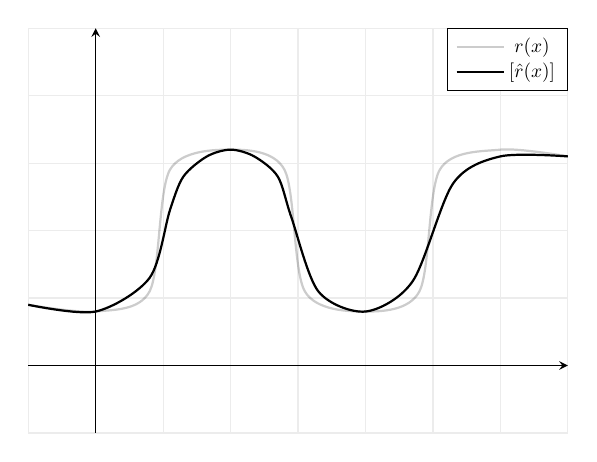
\begin{tikzpicture}[scale=1]
		\begin{axis}[
			ticks=none,
			xtick distance=1,
			ytick distance=1,
			axis equal image=true,
			grid,
			grid style={gray!15},
			grid=both,
			axis lines=middle,
			xmin=-1, xmax=7, ymin=-1, ymax=5,
			axis x line=center,
			axis y line=center,
			legend style={nodes={scale=0.7}, at={(1,1)},anchor=north east}
			]
			\addplot[thick, smooth, opacity = 0.2] plot coordinates
			{
				(-1,0.9) 
				(0,0.8) 
				(0.8, 1.1) 
				(1.1, 2.9) 
				(2, 3.2)
				(2.8, 2.9)
				(3.1, 1.1)
				(4, 0.8) 
				(4.8, 1.1)
				(5.1, 2.9)
				(6, 3.2)
				(7, 3.1)
			};
			\addlegendentry{$r(x)$}
			
			\addplot[thick, smooth] plot coordinates
			{
				(-1,0.9) 
				(0,0.8) 
				(0.8, 1.3) 
				(1.1, 2.3)
				(1.3, 2.8)
				(1.65, 3.1)
				(2, 3.2)
				(2.35, 3.1)
				(2.7, 2.8)
				(2.9, 2.2)
				(3.3, 1.1)
				(4, 0.8) 
				(4.7, 1.25)
				(5.3, 2.7)
				(6, 3.1)
				(7, 3.1)
			};
			\addlegendentry{$\E[\hat r(x)]$}
			
		\end{axis}
		
	\end{tikzpicture}
\end{center}

To compute the variance of $\hat r(x)$, assume the $\xi_i$ are independent with mean 0 and variance $\sigma^2$. Then
\begin{align}
	\text{Var}(\hat r(x)) &= \text{Var}\bigg(\frac{\sum_{i=1}^n w_j Y_j}{\sum_{i=1}^n w_j}\bigg) = \frac{1}{\left(\sum_{j=1}^n w_j\right)^2} \sum_{j=1}^n w_j^2 \text{Var}(Y_j) = \left(\frac{\sum_{j=1}^n w_j^2}{\left(\sum_{j=1}^n w_j\right)^2}\right)\sigma^2.
\end{align}
Let us compute the value of the variance in the case of local averaging. Recall that the kernel used for local averaging is the Boxcar kernel: $w_j = \mathbbm{1}\{|x_j - x| \leq h\}$, so that $(w_1, \ldots, w_n) = (0, \ldots, 0, 1, \ldots, 1, 0, \ldots, 0)$, where the number of 1's is equal to the number of elements that are at most a distance of $h$ from $x$. \\
Suppose we take $x = x_i$. %Let $n_{x_i}$ denote the number of $j$'s such that $|x_j - x_i| \leq h$. Then 
Let $B_{x_i} = \{x_j \colon |x_j - x_i| \leq h\}$ and let  $n_{x_i} = |B_{x_i}|$. Then
\begin{align}
	\text{Var}(\hat r(x_i)) &= \left(\frac{\sum_{j=1}^n w_j^2}{\left(\sum_{j=1}^n w_j\right)^2}\right)\sigma^2 = \left(\frac{\sum_{x_j \in B_{x_i}} 1^2}{\left(\sum_{x_j \in B_{x_i}} 1\right)^2}\right)\sigma^2 = \left(\frac{n_{x_i}}{n_{x_i}^2}\right)\sigma^2 = \frac{\sigma^2}{n_{x_i}}.
\end{align}
We thus see that, in the case of local averaging, the variance of $\hat r(x_i)$ decreases as a function of the number of points in the neighborhood of $x_i$. As $h \to \infty$, the number of points being averaged over increases. So $h = \infty$ gives the smallest possible variance of $\frac{\sigma^2}{n}$ and $h = 0$ gives the largest variance of $\sigma^2$. 

\subsec{Case studies}
Consider the constant function $r(x) = c$ shown below.
\begin{center}
	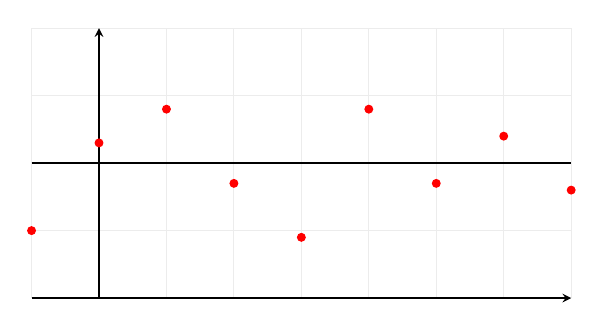
\begin{tikzpicture}[scale=1]
		\begin{axis}[
			ticks=none,
			xtick distance=1,
			ytick distance=1,
			axis equal image=true,
			grid,
			grid style={gray!15},
			grid=both,
			axis lines=middle,
			xmin=-1, xmax=7, ymin=1, ymax=5,
			axis x line=center,
			axis y line=center,
			]
			\addplot[thick, smooth] plot coordinates
			{
				(-1, 3)
				(1, 3)
				(3, 3)
				(5, 3)
				(7, 3)
			};
			\addplot[only marks, color=red, mark options={scale=0.7}] plot coordinates
			{
				(-1, 2)
				(0, 3.3)
				(1, 3.8)
				(2, 2.7)
				(3, 1.9)
				(4, 3.8)
				(5, 2.7)
				(6, 3.4)
				(7, 2.6)
			};
		\end{axis}
	\end{tikzpicture}
\end{center}
Because $r(x)$ is a constant function, bias will be equal to 0 for any choice of $h$ ($\Exp[\hat r(x)] = \frac{\sum_{i=1}^n w_i r(x_i)}{\sum_{i=1}^n w_i} = \frac{\sum_{i=1}^n w_i c}{\sum_{i=1}^n w_i} = c$, so that $\Exp[\hat r(x)] = c = r(x)$ for any choice of kernel and $h$). However, the variance is sensitive to the bandwidth. In this case, we should pick $h = \infty$ to minimize variance and thus minimize MSE. \\

\par Next, let $r(x)$, and the observed data points, be as shown below. Note that $r(x)$ fluctuates quite substantially but the observed points have no noise $(\sigma = 0)$.
\begin{center}
	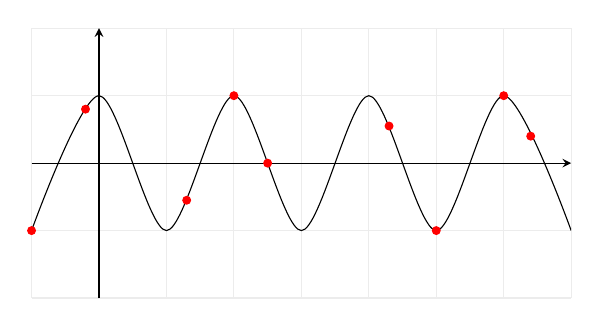
\begin{tikzpicture}[scale=1]
		\begin{axis}[
			ticks=none,
			xtick distance=1,
			ytick distance=1,
			axis equal image=true,
			grid,
			grid style={gray!15},
			grid=both,
			axis lines=middle,
			xmin=-1, xmax=7, ymin=-2, ymax=2,
			axis x line=center,
			axis y line=center,
			]
			\addplot[smooth] plot coordinates
			{
				(-1, -1)
				(0, 1)
				(1, -1)
				(2, 1)
				(3, -1)
				(4, 1)
				(5, -1)
				(6, 1)
				(7, -1)
			};
			\addplot[only marks, color=red, mark options={scale=0.7}] plot coordinates
			{
				(-1, -1)
				(-0.2, 0.8)
				(1.3, -0.55)
				(2, 1)
				(2.5, 0)
				(4.3, 0.55)
				(5, -1)
				(6, 1)
				(6.4, 0.4)
			};
		\end{axis}
	\end{tikzpicture}
\end{center}
In this case, variance = $\frac{\sum_{j=1}^n w_j^2}{\left(\sum_{j=1}^n w_j\right)^2}\sigma^2 = 0$ for all $h$. However, because the function fluctuates, the choice of bandwidth has a large effect on the bias, as it effects how ``smooth'' our estimates will be. Thus, in this case, the  bandwidth should be chosen to minimize bias, i.e. $h = 0$. 
\\
\par Finally, consider the function from the beginning of this lecture, shown again below. 
\begin{center}
	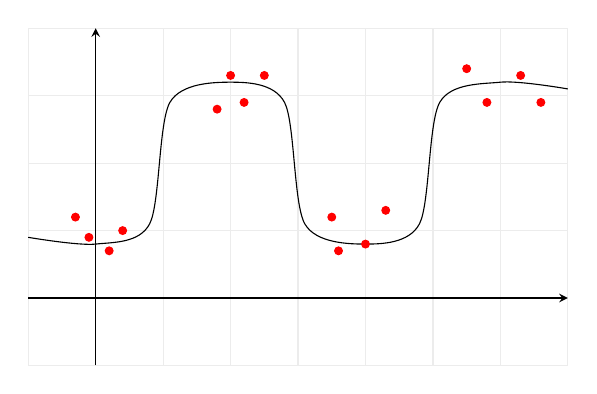
\begin{tikzpicture}[scale=1]
		\begin{axis}[
			ticks=none,
			xtick distance=1,
			ytick distance=1,
			axis equal image=true,
			grid,
			grid style={gray!15},
			grid=both,
			axis lines=middle,
			xmin=-1, xmax=7, ymin=-1, ymax=4,
			axis x line=center,
			axis y line=center,
			]
			\addplot[smooth] plot coordinates
			{
				(-1,0.9) 
				(0,0.8) 
				(0.8, 1.1) 
				(1.1, 2.9) 
				(2, 3.2)
				(2.8, 2.9)
				(3.1, 1.1)
				(4, 0.8) 
				(4.8, 1.1)
				(5.1, 2.9)
				(6, 3.2)
				(7, 3.1)
			};
			\addplot[only marks, color=red, mark options={scale=0.7}] plot coordinates
			{
				(-0.1, 0.9)
				(0.2, 0.7)
				(-0.3, 1.2)
				(0.4, 1)
				
				(2, 3.3)
				(2.2, 2.9)
				(1.8, 2.8)
				(2.5, 3.3)
				
				(3.6, 0.7)
				(3.5, 1.2)
				(4, 0.8)
				(4.3, 1.3)
				
				(5.5, 3.4)
				(5.8, 2.9)
				(6.3, 3.3)
				(6.6, 2.9)
			};
		\end{axis}
		
	\end{tikzpicture}
\end{center}
As discussed in section 2, it is desirable to pick a value of $h$ between 0 and $\infty$, because we would like to average over the noise in the dataset (decrease variance) without smoothing our estimate too substantially (which would increase bias). 

\subsec{Effect of dataset size on bias-variance trade-off}
In general, when we have more data, we can assume that there will be more observations within a given neighborhood of $x$. Because variance depends on the number of data points being averaged over, this means that increasing the number of observations will decrease variance. However, note that Bias$(\hat r(x)) = \frac{1}{n}\sum_{i=1}^m (\Exp[\hat r(x_i)] - r(x))^2$ depends only on the estimator's performance on the clean data, not on the noise in the dataset. Thus, increasing the number of observations does not change the bias. 

Suppose you were at a ``sweet spot'' with the bias-variance trade-off. Then, you observe more data points. This has the effect of decreasing variance while keeping bias constant. Thus, to ``rebalance'' the bias and variance, you should decrease $h$ slightly as to decrease the bias and increase the variance.

\subsec{Formal theorem (bias-variance characterization)} 
We now make the previous discussions of the bias-variance trade-off in the context of kernel estimators more precise with a formal theorem.  While the MSE of an estimator does not depend on the noise in the dataset, it does depend on the (arbitrary) positions of $x_1, \ldots, x_n$. For theoretical feasibility, we assume $x_1, \ldots, x_n \iid P$, where $P$ has density $f(x)$.
Additionally, the theorem has the following setup:
\begin{itemize}
	\item Assume we have an estimator $\hat r_n$ with $n$ samples and that $n$ tends to $\infty$.
	\item For a fixed $n$, the bandwidth is $h_n$.
	\item We use integrated risk to measure the quality of an estimator: $R(\hat r_n, r) \stackrel{\Delta}{=} \int (\hat r_n(x) - r(x))^2 dx$
\end{itemize}
\begin{theorem}
	The risk of a Nadaraya-Watson kernel estimator is
	\begin{align}
		R(\hat r_n, r) &= \colorboxed{blue}{\frac{h_n^4}{4}\left(\int x^2 K(x) dx\right)^2 \int \left(r''(x) + 2r'(x) \frac{f'(x)}{f(x)} \right)^2 dx} \\ &+\colorboxed{red}{\sigma^2 \frac{\int K(x)^2 dx}{nh_n}\left(\int \frac{1}{f(x)}dx\right)} \\
		&+\colorboxed{green}{o\left((nh_n)^{-1}\right)+ o\left(h_n^4\right)}.
	\end{align}
	The term in blue is the \textcolor{blue}{bias} of the estimator and the term in red is the \textcolor{red}{variance}. The terms in \textcolor{green}{green} are higher order terms that go to 0 as $nh_n \to \infty$ and $h_n \to 0$.
\end{theorem} 

We will next try to decompose this theorem to understand each of the individual parts. 

\paragraph{Bias} The theorem tells us that the bias depends on the following quantities: 
\begin{itemize}
	\item bandwidth $h_n$: The smaller the bandwidth, the lower the bias. 
	\item $\int x^2 K(x) dx$: This quantity is a measure of how flat the kernel is. The flatter the kernel, the larger the value of $\int x^2K(x) dx$ and thus the higher the bias. This aligns with our intuition, as the flatter the kernel, the more we are weighting further away points and thus the more smooth our estimator. 
	\item $r''(x)$: This is a measure of the curvature of $r(x)$. The smoother the function, the lower the value of $r''(x)$ and thus the lower the bias. 
	\item $r'(x)\frac{f'(x)}{f(x)}$: Note that this quantity is equal to $r'(x)(\log f(x))'$. This term is called the \textbf{design bias} because it depends on the ``design'' (i.e., the distribution of the $x_i$'s). The design bias is small when $(\log f(x))'$ is small (i.e., when the density of $X$ doesn't change too quickly, or $X$ is ``close to uniform''). 
\end{itemize}

\paragraph{Variance} According to the theorem, the variance depends on the following quantities:
\begin{itemize}
	\item $\sigma^2$: The larger the value of $\sigma^2$ (i.e. the variance of the random noise), the higher the variance. 
	\item $h_n$: The higher the bandwidth, the lower the variance.
	\item $n$: The larger the value of $n$, the smaller the smaller the variance.
\end{itemize}

\paragraph{Implications on bandwidth $h_n$}
Let us treat $K, f,$ and $r$ as constants. We are interested in seeing how the optimal bandwidth $h_n^*$ changes as a function of $\sigma^2$ and $n$. Holding $K, f,$ and $r$ constant, we can express the risk as 
\begin{equation} R(\hat r(x), r(x)) = h_n^4 c_1 + \frac{\sigma^2}{nh_n}c_2 + \text{higher order terms,}\end{equation} 
where $c_1$ and $c_2$ are constants. We are thus interested in the choice of $h_n$ that minimizes this risk. By taking the derivative of the risk and setting it equal to zero, we see that
\begin{equation}
	h_n^* = c_3\left(\frac{\sigma^2}{n}\right)^{1/5}.
\end{equation}
This tells us that the optimal bandwidth decreases at a rate proportional to $n^{-1/5}.$ 

Plugging in $h_n^*$ to the risk equation, we see that \begin{equation}
	\underset{h_n}{\text{min}}\left(h_n^4 c_1 + \frac{\sigma^2 c_2}{nh_n}\right) = c_4 \left(\frac{\sigma^2}{n}\right)^{4/5},
\end{equation}
so that the lowest risk is on the order of $n^{-4/5}$. Note that the risk for most parametric models is on the order of $n^{-1}$, a slight improvement over the risk for the nonparametric models we have discussed. 

\sec{Linear smoothers: a unified view}
We now take a brief detour to introduce the concept of linear smoothers, which serve as a way to unify many of the aforementioned nonparametric regression methods.
\begin{definition}
	$\hat r$ is a \textbf{linear smoother} if there exists a vector valued function $x \longrightarrow (l_1(x), \ldots, l_n(x))$ such that 
	\begin{equation}
		\hat r(x) = \sum_{i=1}^m l_i(x)Y_i.
	\end{equation}
\end{definition} 
Note that the $l_i$'s can depend on $x_1, \ldots, x_n$ but not on $Y_1, \ldots, Y_n$. Additionally, we must have that $\sum_{i=1}^n l_i(x) = 1$.
\begin{prop} 
	The regressogram and kernel estimator are both instances of linear smoothers. 
	\begin{itemize}
		\item Regressogram:
		\begin{align}
			\hat r(x) &= \frac{1}{|B_x|}\sum_{i \in B_x} Y_i = \sum_{i=1}^n \left(\frac{\mathbbm{1}\{x_i \in B_x \}}{|B_x|}\right) Y_i = \sum_{i=1}^m l_i(x)Y_i,
		\end{align}
		where $B_x$ is the bin containing $x$ and $l_i(x) = \frac{\mathbbm{1}\{x_i \in B_x\}}{|B_x|}$.
		\item Kernel estimator:
		\begin{align}
			\hat r(x) &= \frac{\sum_{i=1}^n w_i Y_i}{\sum_{i=1}^n w_i} = \sum_{i=1}^n \left(\frac{w_i}{\sum_{j=1}^n w_j}\right)Y_i = \sum_{i=1}^m l_i(x)Y_i,
		\end{align}
		where $l_i(x) = \frac{w_i}{\sum_{j=1}^n w_j}$
	\end{itemize}
\end{prop}
Thus, linear smoothers provide a ``unified view'' in that they provide a category into which many different types of estimators fall. In the next section, we will introduce the method of local linear regression, which we show is yet another instance of a linear smoother. We now conclude this section with a few facts about linear smoothers. 
\begin{itemize}
	\item We can write any linear smoother in the matrix multiplication form $\hat{\bm{r}} = \bm L \bm Y$, where 
	$\hat{\bm{r}} = 
	\begin{bmatrix}
		\hat r_1(x) \\
		\vdots \\
		\hat r_n(x)
	\end{bmatrix}$, $\bm L = \begin{bmatrix}
		l_1(x_1) & \cdots & l_n(x_1) \\
		\vdots & \ddots & \vdots\\
		l_1(x_n) & \cdots & l_n(x_n), 
	\end{bmatrix}$, and $\bm Y = \begin{bmatrix}
		Y_1 \\
		\vdots \\
		Y_n
	\end{bmatrix}$.
	\item For all linear smoothers, 
	\begin{align}
		\Exp[\hat r(x)] &= \Exp\big[\sum_{i=1}^n l_i(x)Y_i\big] =  \sum_{i=1}^n l_i(x) \Exp[Y_i] = \sum_{i=1}^n l_i(x)r(x),
	\end{align}
	so $\Exp[\hat r(x)]$ is equal to the estimate when the estimator is run on clean data. Like in the particular case of kernel estimators, the bias is an indicator of how much we damage the clean data by smoothing. 
\end{itemize}
\sec{Local linear regression}
Local linear regression provides an alternative to kernel estimators. To motivate why we might want such an alternative, let us revisit the idea of design bias. Consider the following function $r(x)$, along with the observed data points, shown below.


\begin{center}
	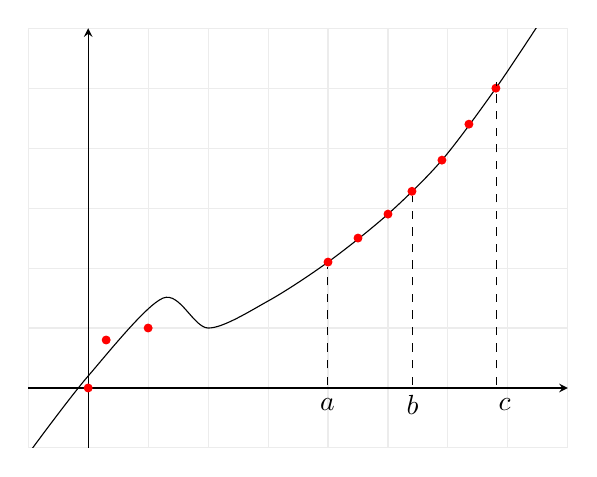
\begin{tikzpicture}[scale=1]
		\begin{axis}[
			ticks=none,
			xtick distance=1,
			ytick distance=1,
			axis equal image=true,
			grid,
			grid style={gray!15},
			grid=both,
			axis lines=middle,
			xmin=-1, xmax=8, ymin=-1, ymax=6,
			axis x line=center,
			axis y line=center,
			]
			\addplot[smooth] plot coordinates
			{
				(-1,-1.1) 
				(0,0.2) 
				(1.25, 1.5) 
				(2, 1) 
				(3, 1.45)
				(4, 2.1)
				(5, 2.9) 
				(5.9,3.8)
				(6.8,5)
				(7.6,6.2)
			};
			\addplot[only marks, color=red, mark options={scale=0.7}] plot coordinates
			{
				(4, 2.1)
				(4.5, 2.5)
				(5, 2.9) 
				(5.4, 3.28)
				(5.9,3.8)
				(6.35, 4.4)
				(6.8,5)
				
				(0, 0.0)
				(0.3, 0.8)
				(1, 1) 
			};
		\end{axis}
		
		\node[] at (3.8,0.55) {$a$};   
		\node[] at (6.05,0.55) {$c$}; 
		\node[] at (4.88, 0.55){$b$};
		%\draw[->] (2.5,3.6) -- (3,2);
		
		\draw[dashed] (4.88,0.8) -- (4.88,3.2);
		\draw[dashed] (3.8,0.8) -- (3.8,2.3);
		\draw[dashed] (5.95,0.8) -- (5.95,4.65);
		
	\end{tikzpicture}
\end{center}

If we were to use a kernel estimator to attempt to predict $r(a)$, we would overestimate the true value. This is because all observed points that are close to $a$ are to the right of $a$, so we would average primarily over points whose $y$-values are larger than $a$'s. The predicted value for $r(a)$ using local averaging is marked in green in the plot below. 

\begin{center}
	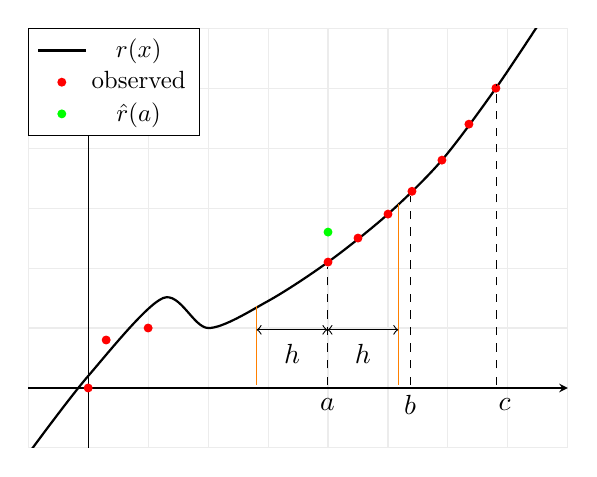
\begin{tikzpicture}[scale=1]
		\begin{axis}[
			ticks=none,
			xtick distance=1,
			ytick distance=1,
			axis equal image=true,
			grid,
			grid style={gray!15},
			grid=both,
			axis lines=middle,
			xmin=-1, xmax=8, ymin=-1, ymax=6,
			axis x line=center,
			axis y line=center,
			legend style={nodes={scale=0.9}, at={(0,1)},anchor=north west}
			]
			\addplot[thick, smooth] plot coordinates
			{
				(-1,-1.1) 
				(0,0.2) 
				(1.25, 1.5) 
				(2, 1) 
				(3, 1.45)
				(4, 2.1)
				(5, 2.9) 
				(5.9,3.8)
				(6.8,5)
				(7.6,6.2)
			};
			\addlegendentry{$r(x)$}
			\addplot[only marks, color=red, mark options={scale=0.7}] plot coordinates
			{
				(4, 2.1)
				(4.5, 2.5)
				(5, 2.9) 
				(5.4, 3.28)
				(5.9,3.8)
				(6.35, 4.4)
				(6.8,5)
				
				(0, 0.0)
				(0.3, 0.8)
				(1, 1) 
			};
			\addlegendentry{observed}
			\addplot[only marks, color=green, mark options={scale=0.7}] plot coordinates
			{
				(4, 2.6)
			};
			\addlegendentry{$\hat r(a)$}
		\end{axis}
		%\node[anchor=west, text width=5cm] at (2,4) {$E[x]$ will be overestimate blah blah};    
		\node[] at (3.35,1.2) {$h$};   
		\node[] at (4.25,1.2) {$h$};
		\node[] at (3.8,0.55) {$a$};   
		\node[] at (6.05,0.55) {$c$}; 
		\node[] at (4.85, 0.55){$b$};
		%\draw[->] (2.5,3.6) -- (3,2);
		
		\draw[dashed] (4.85,0.8) -- (4.85,3.2);
		\draw[dashed] (3.8,0.8) -- (3.8,2.3);
		\draw[dashed] (5.95,0.8) -- (5.95,4.62);
		
		\draw[color=orange] (2.9,0.8) -- (2.9,1.8);
		\draw[color=orange] (4.7,0.8) -- (4.7,3.1);
		
		%\draw [decorate,decoration = {brace,amplitude=5pt,mirror}] (2.9,0.4) -- (3.8,0.4);
		\draw[<->] (2.9,1.5) -- (3.8,1.5);
		\draw[<->] (3.8,1.5) -- (4.7,1.5);
	\end{tikzpicture}
\end{center}

Similarly, using a kernel estimator to predict $r(c)$ would result in an underestimate. In contrast, because $b$ has nearby points on either side, the prediction for $r(b)$ would be reasonable. This problem of over/underestimating $r(x)$ for points that have no observations on one side (i.e. points on the boundary of a given bin) is closely related to the design bias. It occurs because, when using kernel estimators, we make the assumption that $r(x)$ is locally constant. 

Local linear regression provides a solution to this problem. Rather than assuming $r(x)$ is locally constant, we assume that $r(x)$ is locally linear. For a given data point $x$, we would like to approximate $r(x)$ by locally fitting a line based at $x$ to our data. Let $\tilde{r}_x(u) = a_1(u - x) + a_0$. Then the algorithm for local linear regression is as follows. 

For a given data point $x$, let \begin{equation}\hat a_0, \hat a_1 = \argmin_{a_0, a_1} \sum_{i=1}^n w_i(Y_i - \tilde{r}_x(x_i))^2 = \argmin_{a_0, a_1} \sum_{i=1}^n w_i(Y_i - (a_1(x_i - x) + a_0))^2,\end{equation}
where $w_i = K\left(\frac{(x_i-x)}{h}\right)$ for some kernel function $K$. Then, we let our estimate $\hat r(x)$ equal the intercept term: 
\begin{equation}
	\hat r(x) \stackrel{\Delta}{=} \hat a_0.
\end{equation}
\begin{theorem} The integrated risk of local linear regression consists of a bias term and variance term. The variance is the same as that from Theorem 1. The bias is \begin{align}
	\frac{h_n^4}{4}\left(\int x^2 k(x) dx\right)^2 \int r''(x)^2 dx.
\end{align}
\end{theorem}
If we compare this bias to the bias from the kernel estimators ($\frac{h_n^4}{4}(\int x^2 k(x) dx)^2 \cdot$ $\int (r''(x) + 2r'(x) \frac{f'(x)}{f(x)})^2dx$), we see that the bias for local linear regression does not have the $2r'(x) \frac{f'(x)}{f(x)}$ term (i.e. no design bias!). Local linear regression thus mitigates the problem of design bias that we encounter when using kernel estimators. The diagram below provides some intuition as to why this is the case.

\begin{center}
	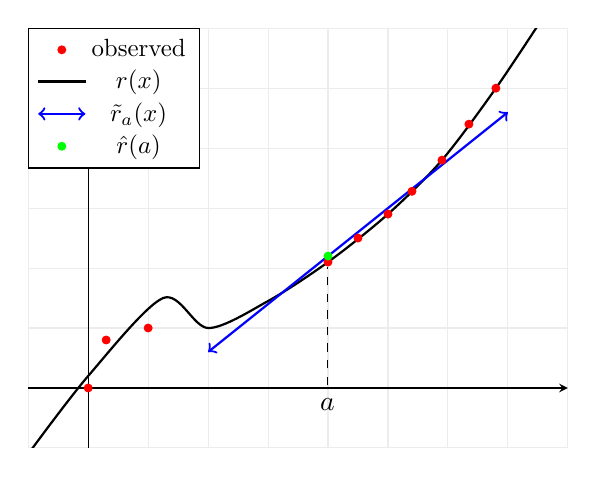
\begin{tikzpicture}[scale=1]
		\begin{axis}[
			ticks=none,
			xtick distance=1,
			ytick distance=1,
			axis equal image=true,
			grid,
			grid style={gray!15},
			grid=both,
			axis lines=middle,
			xmin=-1, xmax=8, ymin=-1, ymax=6,
			axis x line=center,
			axis y line=center,
			legend style={nodes={scale=0.9}, at={(0,1)},anchor=north west}
			]
			\addplot[only marks, color=red, mark options={scale=0.7}] plot coordinates
			{
				(4, 2.1)
				(4.5, 2.5)
				(5, 2.9) 
				(5.4, 3.28)
				(5.9,3.8)
				(6.35, 4.4)
				(6.8,5)
				
				(0, 0.0)
				(0.3, 0.8)
				(1, 1) 
			};
			\addlegendentry{observed}
			
			\addplot[thick, smooth] plot coordinates
			{
				(-1,-1.1) 
				(0,0.2) 
				(1.25, 1.5) 
				(2, 1) 
				(3, 1.45)
				(4, 2.1)
				(5, 2.9) 
				(5.9,3.8)
				(6.8,5)
				(7.6,6.2)
			};
			\addlegendentry{$r(x)$}
			\addplot[<->, thick, smooth, color=blue] plot coordinates
			{
				(2, 0.6)
				(3, 1.4)
				%(3.5, 1.7)
				%(4, 2.1)
				%(4.5, 2.5)
				%(5, 2.9)
				%(5.5, 3.4)
				%(6, 3.8)
				(7, 4.6)
			};
			\addlegendentry{$\tilde r_a(x)$}
			
			\addplot[only marks, color=green, mark options={scale=0.7}] plot coordinates
			{
				(4, 2.2)
			};
			\addlegendentry{$\hat r(a)$}
		\end{axis}
		%\node[anchor=west, text width=5cm] at (2,4) {$E[x]$ will be overestimate blah blah};   
		\node[] at (3.8,0.55) {$a$};   
		%\draw[->] (2.5,3.6) -- (3,2);
		
		\draw[dashed] (3.8,0.8) -- (3.8,2.3);
		
		%\draw [decorate,decoration = {brace,amplitude=5pt,mirror}] (2.9,0.4) -- (3.8,0.4);
	\end{tikzpicture}
\end{center}

We see that the local linear assumption allows us to better approximate $r(x)$ for values of $x$ that lie on the boundary. We conclude by proving that local linear regression is another instance of a linear smoother.
\begin{align*}
	\hat a_0, \hat a_1 &= \argmin_{a_0, a_1} \sum_{i=1}^n w_i(Y_i - (a_1(x_j - x) + a_0))^2 = \argmin_{a_0, a_1} \hspace{0.2cm} g(a_0, a_1). \\
	\frac{\partial g}{\partial a_0} &= 2 \sum_{i=1}^n w_i(a_1 (x_i - x) + a_0 - Y_i) = 0 \\
	\frac{\partial g}{\partial a_1} &= 2 \sum_{i=1}^n w_i(a_1 (x_i - x) + a_0 - Y_i)(x_i - x) = 0.
\end{align*}
By solving this system of equations for $a_0$ and $a_1$, we get that 
\begin{equation}
	\hat r(x) = \hat a_0 = \frac{\sum_{i=1}^n (w_i C Y_i - w_i (x_i - x)B Y_i)}{AC-B^2} = \sum_{i=1}^n \left(\frac{w_iC - w_i(x_i-x)B}{AC-B^2} \right)Y_i,
\end{equation}
where $A = \sum_{i=1}^n w_i$, $B =  \sum_{i=1}^n w_i (x_i - x)$ and $C =  \sum_{i=1}^n w_i (x_i - x)^2$. We thus see that $\hat r(x)$ is a linear combination of the $Y_i$'s, so local linear averaging is indeed a linear smoother. 